\documentclass{article}

\usepackage{amsmath,amsfonts,amsthm,amssymb}
\usepackage{fancyhdr}
\usepackage{float}
\usepackage{lastpage}
\usepackage{graphicx}
\usepackage{supertabular}
\usepackage{multirow}
\usepackage{ifthen}
\usepackage{enumerate}
\usepackage{subcaption}
\usepackage[hidelinks]{hyperref}
\usepackage{soul}

% In case you need to adjust margins:
\topmargin=-0.5in
\evensidemargin=0in
\oddsidemargin=0in
\textwidth=6.5in
\textheight=9.0in
\headsep=0.25in

% Homework Specific Information
\newcommand{\hmwkTitle}{Project Report 3}
\newcommand{\hmwkDueDate}{April 9th, 2014}
\newcommand{\hmwkClass}{42-731}
\newcommand{\hmwkAuthor}{Alex Sun Yoo, Michael Nye, Ozan Iskilibli}
\newcommand{\hmwkEmail}{ayoo, mnye, oiskilib}
\newcommand{\hmwkCollaborators}{}
\newcommand{\bigspace}{\vspace{.25in}}

% Tools for formatting questions
\newcommand{\question}[1] {\vspace{.25in} \hrule\vspace{0.5em}
\noindent{\bf #1} \vspace{0.5em}
\hrule \vspace{.10in}}
\renewcommand{\part}[1] {\vspace{.10in} {\bf (#1)}}

% Setup the header and footer
\pagestyle{fancyplain}
\lhead{\fancyplain{}{\hmwkAuthor \\ \hmwkEmail}}
\chead{\fancyplain{}{\textbf{\hmwkTitle}}}
\rhead{\fancyplain{}{\hmwkClass \\ Due:\ \hmwkDueDate}}
\lfoot{}
\cfoot{}
\rfoot{Page\ \thepage\ of\ \pageref{LastPage}}
\renewcommand\headrulewidth{0.4pt}
\renewcommand\footrulewidth{0.4pt}

% Format paragraphs to have spacing instead of indents
\setlength{\parindent}{0pt}
\setlength{\parskip}{5pt plus 1pt}

% This is used to trace down (pin point) problems
% in latexing a document:
%\tracingall

\renewcommand{\arraystretch}{1.5}

%%%%%%%%%%%%%%%%%%%%%%%%%%%%%%%%%%%%%%%%%%%%%%%%%%%%%%%%%%%%%

\begin{document}

\thispagestyle{plain}
\begin{center}
{\Large \hmwkClass\ \hmwkTitle} \\
\hmwkAuthor \\
\hmwkEmail \\
\ifthenelse{\equal{\hmwkCollaborators}{}}{}{Collaborators: \hmwkCollaborators\\}
Due: \hmwkDueDate\\
\end{center}
%%%%%%%%%%%%%%%%%%%%%%%%%%%%%%%%%%%%%%%%%%%%%%%%%%%%%%%%%%%%%

\section*{Part 1: Microscope Characterization}

\subsection*{B.1 Image Data}

All of our image data is read into a vector of structs, with consistent field naming. This allows us to write generic functions that can operate on any set of images we pass to it, and gives us a grouping with which to store all results bundled together.


\subsection*{B.2 Characterizing fluorescence image background noise}

To compute noise statistics, we first crop out a region of the image containing noise. To do so, a region in each image that contained no features was manually found, and then that region was stored into our script for repeatability. Each image is then cropped using this region, and the mean and variance is calculated over the cropped region.

To determine the distribution of the data, the noise samples were plotted in a histogram and inspected visually. Upon observation, it was found that the data appears to perfectly follow a Gaussian distribution, shown in Figure \ref{fig:noise_dist_background}.

To analyze the image sequence over time, we then generated plots showing the mean and variance of the noise over time for the image sequence. We found that both the mean and variance of the noise intensity decreased over time, shown in Figure \ref{fig:noise_mean_var_time}.

To analyze the spatial dependency of the noise, we plotted the mean of noise over columns in one plot, and rows in another (Figure \ref{fig:noise_intensity_space}. We found that the intensity was highest for our noise field in the top left, and lowest in the bottom right. The noise displays a rough linear decay across the image in both the $x$ and $y$ directions.

% TODO: FIGURES

\begin{figure}[b]
\begin{minipage}[b]{0.45\linewidth}
\centering
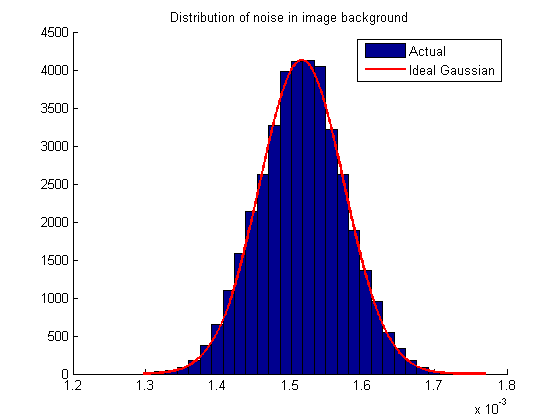
\includegraphics[width=\textwidth]{figures/noise_distribution_background.png}
\caption{Noise distribution in background}
\label{fig:noise_dist_background}
\end{minipage}
\hspace{0.5cm}
\begin{minipage}[b]{0.45\linewidth}
\centering
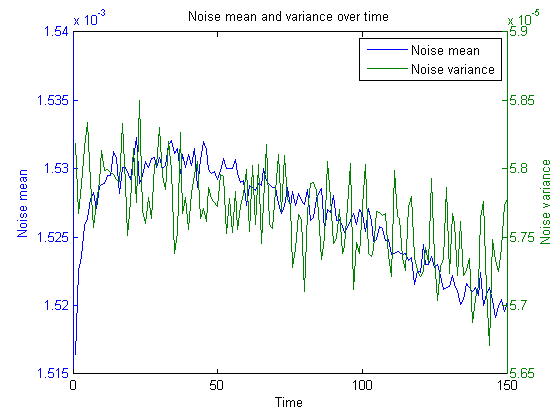
\includegraphics[width=\textwidth]{figures/noise_mean_variance_over_time.png}
\caption{Noise Mean \& Variance over time}
\label{fig:noise_mean_var_time}
\end{minipage}
\end{figure}

\begin{figure}[t]
\centering
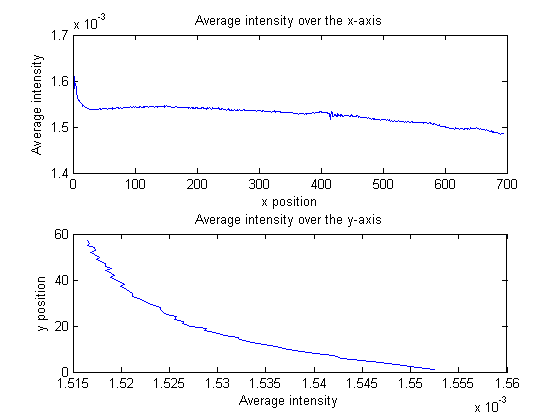
\includegraphics[width=0.45\linewidth]{figures/noise_intensity_over_space.png}
\caption{Average Noise Intensity over Space}
\label{fig:noise_intensity_space}
\end{figure}


\subsection*{B.3 Characterizing illumination uniformity}



\subsection*{B.4 Microscope pixel calibration}
 


\subsection*{B.5 Implementation of a directional anisotropic filter}



\pagebreak
\section*{Part 2: Curvilinear feature detection}

\subsection*{C.1 Implementation of the Steger's algorithm}



\subsection*{C.2 Implementation of the pixel inking operation}



\pagebreak
\begin{thebibliography}{9}
\fontsize{10pt}{12pt}\selectfont
\raggedright

    \bibitem{steger}
        C. Steger, An unbiased detector of curvilinear structures, 
        \emph{IEEE Trans. Pattern Analysis and Machine Intelligence},
        vol. 20, pp. 113-125, 1998.

    \bibitem{geusebroek}
        J. M. Geusebroek, A. W. M. Smeulders, and J. van de Weijer, 
        \ul{Fast anisotropic Gaussian filtering},
        \emph{IEEE Trans. Image Processing}, vol. 12, no. 8, pp. 938-943, 2003.


\end{thebibliography}


%%%%%%%%%%%%%%%%%%%%%%%%%%%%%%%%%%%%%%%%%%%%%%%%%%%%%%%%%%%%%

\end{document}

%%%%%%%%%%%%%%%%%%%%%%%%%%%%%%%%%%%%%%%%%%%%%%%%%%%%%%%%%%%%%
